\section{Experimental Evaluation}\label{sec:evaluation}

An Acting system, the Robustness Heuristics and the Task Perparations were implemented directly inside the system Fape \citep{bit-monnotFAPEConstraintbasedPlanner2020}.
The Statement around Fape supporting acting made in \cite{bit-monnotTemporalHierarchicalModels2016a} were not present in the current system as they have apperently only been discussed theoretically or parts were deleted because of the domain dependent implementation.
Due to technical difficulties, planning of tasks by interleaving with already planned tasks and replanning could not be implemented in time.
Evaluation regarding these parts is done manually.

The evaluation was done in an LXC container with 12 Intel(R) Xeon(R) Gold 6334 CPU 3.60GHz Cores, 32 GB RAM.
The planning itself is however a single threaded process, so only one CPU Core can be used.

It has to be mentioned that Fape is not the most performant HTN planner, but besides CHIMP the only one supporting all required features.

Quantitative Metrics:
Plan time
Search Nodes
Average Branching Factor

Makespan/Duration

Qualitative Metrics:
Success

Possible Comparisons:
HTN PO vs HTN TO vs Classical \citep{yuxinliuPlanningOvercookedGame2020}
HTN vs HTN + Robustness
HTN Oracle vs HTN Acting vs HTN Acting + Robustness vs HTN + Preparations


\subsection{HTN vs Classical Planning in Overcooked}

\bild{fig:eval-mapB}{pddl_mapB}{Map}{10}

In this section, we compare our HTN domain definition for ``Overcooked'' with the PDDL domain definition by \cite{yuxinliuPlanningOvercookedGame2020}.
It is not possible to directly compare the makespan between the domains, as not all of the action durations were provided.
To plan using the HTN domain definition, we use FAPE \citep{bit-monnotTemporalHierarchicalModels2016a} and they use the Temporal Fast Downward planner \citep{eyerichUsingContextenhancedAdditive2009}.
The problem considered is the ``Map B'' from \cite{yuxinliuPlanningOvercookedGame2020} shown in figure \ref{fig:eval-mapB}.
They call it a complex map, as it incentivizes the cooks to use the counters for faster transportation.
The goal of this problem is to prepare either one or two burgers with two cooks.


We consider four different variants of our domain:
\begin{itemize}
  \item Full Hier.: All action templates are task-dependent and the duration of the action template \verb|a_move| is fixed at 5.
  \item Full Hier. + Dur: All action templates are task-dependent and the duration of the action template \verb|a_move| is the shortest distance in the map calculated using the A* search algorithm. 
  \item Part. Hier.: The action template \verb|a_move| is not task-dependent, so agents can move freely in the domain if necessary and the duration of the action template \verb|a_move| is fixed at 5.
  \item Part. Hier. + Dur: The action template \verb|a_move| is not task-dependent, so agents can move freely in the domain if necessary and the duration of the action template \verb|a_move| is the shortest distance in the map calculated using the A* search algorithm. 
\end{itemize}

It is important to note that FAPE uses different heuristics by default during planning compared to TFD.
FAPE uses the heuristic minimal spanning tree for partially hierarchical domains and depth-first search in fully hierarchical domains.
While the selection of different heuristics is possible in FAPE, it is not considered in this comparison.
\cite{yuxinliuPlanningOvercookedGame2020} uses the shortest makespan heuristic.
As such, FAPE only does satisficing while TFD tries to find the optimal plan.

Additionally, TFD uses State-Space search while FAPE uses Plan-Space search.
This makes the generated nodes not directly comparable.

The results of planning the delivery of one burger are shown in Table \ref{tab:eval-burger}.
TFD is faster in the generation of the plan and visits significantly more nodes than FAPE.
The search time for the partial hierarchy is also slower than the fully hierarchal version.
The inclusion of the representative movement durations also increases the search time for both variants.
The makespan is however shorter for the partial hierarchy compared to the full hierarchy, especially when using the representative movement durations.


\begin{table}
  \begin{tabular}{lcllll}
                   & Success & search time  & generated nodes & makespan         \\
    \hline
    TFD             & yes & $20s$            &  10546          &  125.1       \\
    Full Hier.            & yes & $31.0s\pm 0.9$   & $125\pm 0.0$    &  $232\pm 0.0$            \\
    Full Hier. + Dur      & yes & $37.9s\pm 1.6$   & $125\pm 0.0$    &  $368\pm 0.0$      \\
    Part. Hier.      & yes & $563.0s\pm 45.1$ & $3754\pm 0.0$   &  $227\pm 0.0$   \\
    Part. Hier. + Dur & yes & $628.0s\pm 16.9$ & $3744\pm 0.5$   &  $318\pm 0.0$            \\
  \end{tabular}
  \caption{Produce one burger}
  \label{tab:eval-burger}
\end{table}

The results for planning the delivery of two burgers are shown in Table \ref{tab:eval-burgers}.
Both planners are unable to find a solution in this case.
TFD does consider more search nodes than FAPE, as in the previous comparison.

\begin{table}
  \begin{tabular}{lcllll}
    & Success & search time  & generated nodes & makespan         \\
  \hline
  TFD             & no & $1000s+$ & 1000000+ &  -       \\
  FAPE            & no & $1000s+$ & 5360+    &  -          \\
  FAPE + Dur      & no & $1000s+$ & 7430+    &  -    \\
  FAPE + TI       & no & $1000s+$ & 3800+    &  - \\
  FAPE + Dur + TI & no & $1000s+$ & 3071+    &  -          \\
  \end{tabular}
  \caption{Produce two burgers}
  \label{tab:eval-burgers}
\end{table}

\subsection{Robustness Heuristic}

In this section, we evaluate the Robustness Heuristic introduced in Section \ref{sec:approach-robustness}.
Heuristics can be provided as a list in FAPE, to assign a priority.
The additional heuristics are used to break ties between previous heuristics.

The default heuristics used are depth-first search (``dfs''), ordered decomposition (``ord-dec'') and ``soca'' which is a simple comparison between the number of flaws and actions.
We compare this default heuristic with four different combinations of adding either the shortest makespan or the robustness heuristic at index 2 or 3.
The depth-first search should always be at the first index for fully hierarchical problems, as the search would otherwise not resolve tasks first.

\bild{fig:eval-overcooked}{overcooked2_tutorial}{Overcooked!2 Tutorial level}{10}

We compare the heuristic combinations in the following four different simple problems.
The environment for the salads is the tutorial level for ``Overcooked!2'' (see Figure \ref{fig:eval-overcooked}).
The burger uses the same environment as in the previous section (see Figure \ref{fig:eval-mapB}).
\begin{enumerate}
  \item a lettuce salad, with a deadline of 150:\\ 
    \verb|[start, start+150] contains order_po_lettuce_salad(client1);|
  \item two lettuce salads, with a deadline of 300 each:\\
    \verb|[start, start+300] contains order_po_lettuce_salad(client1);|\\
    \verb|[start, start+300] contains order_po_lettuce_salad(client2);|\\
  \item a tomato salad with a deadline of 200:\\
    \verb|[start, start+200] contains order_po_lettuce_tomato_salad(client1);|
  \item a burger with a deadline of 200:\\
    \verb|[start, start+400] contains order_po_lettuce_tomato_burger(client1);|
\end{enumerate}

The results are shown in table \ref{tab:eval-heuristics}.
Producing a single sala takes only around 10 seconds for all of the heuristics.
The makespan heuristic combinations achieve a significant decrease in the makespan of the plan.
The makespan of the robustness heuristics is not better than the default and has a high standard deviation.
None of the heuristics can provide a plan for two salads at once in under 1000 seconds.





% Please add the following required packages to your document preamble:
% \usepackage{multirow}
% Please add the following required packages to your document preamble:
% \usepackage{multirow}
% Please add the following required packages to your document preamble:
% \usepackage{multirow}
\begin{table}[]
  \begin{tabular}{p{1.5cm}rrrrr}
  \multicolumn{1}{l}{}         & \multicolumn{1}{l}{heuristic} & success & \multicolumn{1}{l}{plantime} & \multicolumn{1}{l}{generated states} & \multicolumn{1}{l}{makespan} \\ \hline \hline
  \multirow{5}{*}{salad}        & default                       & yes     & $11.8s\pm1.5 $              & $46.0\pm0.0$                         & $115.0 \pm0.0$               \\ 
                                & makespan@2                    & yes     & $11.4s\pm1.5 $              & $53.0\pm0.0$                         & $79.0  \pm0.0$               \\ 
                                & makespan@3                    & yes     & $11.1s\pm1.7 $              & $53.0\pm0.0$                         & $79.0  \pm0.0$               \\
                                & robustness@2                  & yes     & $11.6s\pm1.3 $              & $48.6\pm5.3$                         & $110.6 \pm25.5$               \\ 
                                & robustness@3                  & yes     & $11.7s\pm1.3 $              & $45.8\pm2.5$                         & $115 \pm21.2$               \\\hline
  \multirow{5}{*}{\parbox{1.2cm}{two salads}}   
                                & default                       & no      & $1000.0s+$                  & $39641.0\pm?$                        & $-     $                     \\
                                & makespan@2                    & no      & $1000.0s+$                  & $38906.2\pm1541.4$                   & $-     $                     \\
                                & makespan@3                    & no      & $1000.0s+$                  & $36023.0\pm554.3$                    & $-     $                     \\
                                & robustness@2                  & no      & $1000.0s+$                  & $16584.0\pm?$                        & $-     $                     \\ 
                                & robustness@3                  & no      & $1000.0s+$                  & $21336.0\pm?$                        & $-     $                     \\\hline
  \multirow{5}{*}{\parbox{1.5cm}{tomato salad}} 
                                & default                       & yes     & $10.8s\pm1.5 $              & $75.0\pm0.0$                         & $180.0 \pm0.0$               \\
                                & makespan@2                    & yes     & $12.0s\pm0.3 $              & $119.0\pm0.0$                        & $118.0 \pm0.0$               \\
                                & makespan@3                    & yes     & $12.0s\pm0.2 $              & $115.0\pm0.0$                        & $121.0 \pm0.0$               \\
                                & robustness@2                  & yes     & $15.0s\pm2.7 $              & $171.4\pm$                           & $175.4 \pm2.2$               \\
                                & robustness@3                  & yes     & $12.1s\pm1.8 $              & $79.2\pm$                            & $190.2 \pm3.9$               \\\hline
  \multirow{5}{*}{burger}       & default                       & yes     & $38.1s\pm 3.1$              & $125.0\pm0.0$                        & $368.0\pm0.0$                \\
                                & makespan@2                    & no      & $1000.0s+$                  & $5389.2\pm448.1$                     & $-     $                     \\
                                & makespan@3                    & no      & $1000.0s+ $                 & $5323.6\pm234.7$                     & $-     $                     \\
                                & robustness@2                  & yes     & $342.1s\pm365.2 $           & $2108.8\pm2462.0$                    & $329.4 \pm21.29$             \\ 
                                & robustness@3                  & 50\%    & $522.5s\pm675.4 $           & $1918.5\pm2535.0$                    & $358.0 \pm?$                                      
  \end{tabular}
  \caption[Performance results for different heuristic combinations]{Performance results for different heuristic combinations on different tasks. The default heuristic is a priority combination with depth-first search (``dfs''), ordered decomposition (``ord-dec'') and ``soca'' which is a simple comparison between the number of flaws and actions. The other heuristic combinations in the table are created by inserting them at the respective index (starting at 1) in the priority combination, e.g. makespan@2 would result in the list (dfs,makespan,ord-dec,soca).}
  \label{tab:eval-heuristics}
\end{table}

\subsection{Acting}

\rotatebox{90}{
  \begin{minipage}{\textheight}
    \begin{minipage}{\textheight}
      \centering
      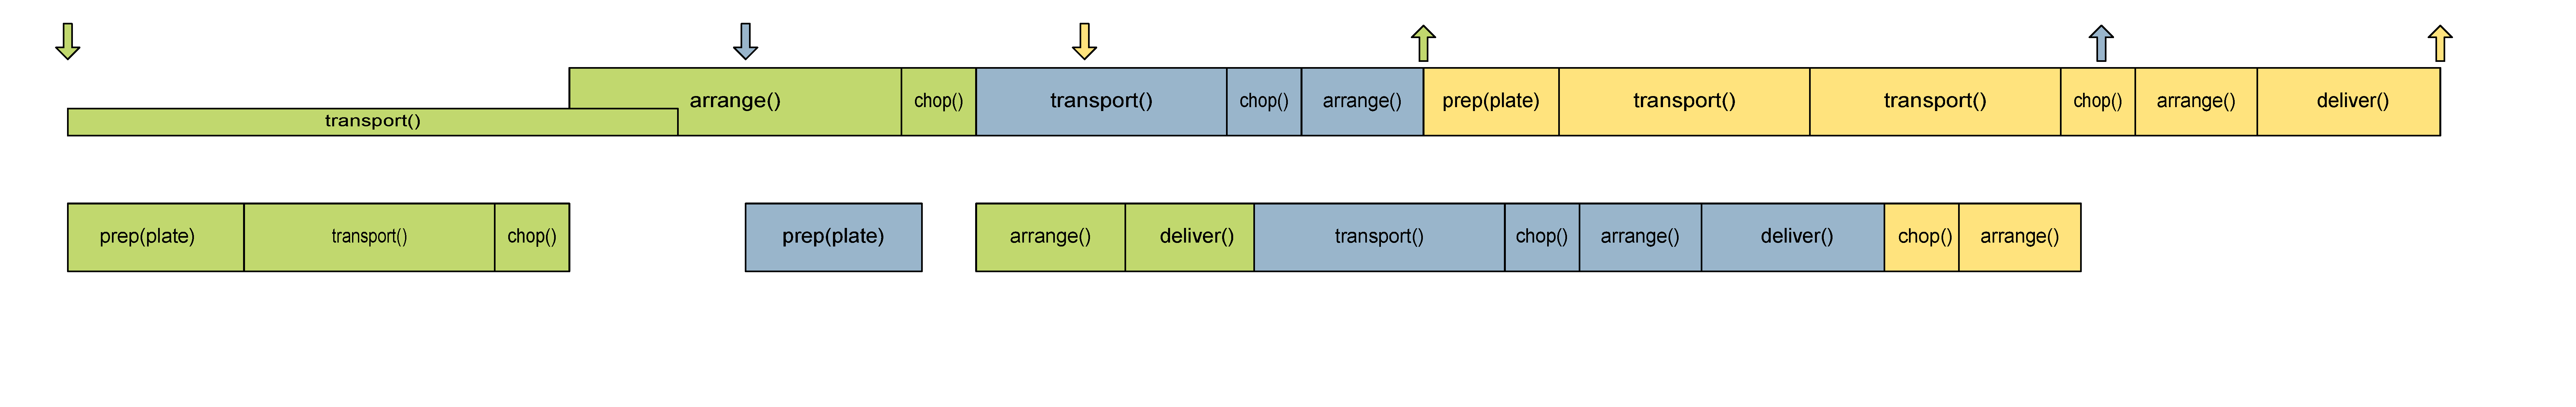
\includegraphics[width=\linewidth]{images/Scenario3 tomato - default.pdf}
    \end{minipage}
    \begin{minipage}{\textheight}
      \centering
      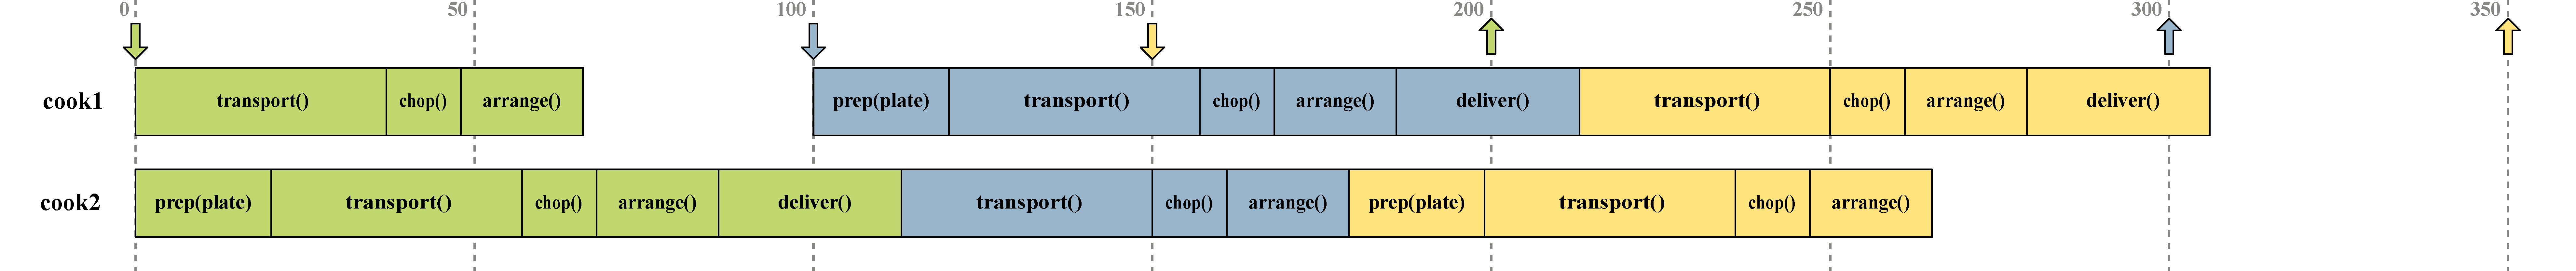
\includegraphics[width=\linewidth]{images/Scenario3 tomato - oracle_makespan.pdf}
    \end{minipage}
    \begin{minipage}{\textheight}
      \centering
      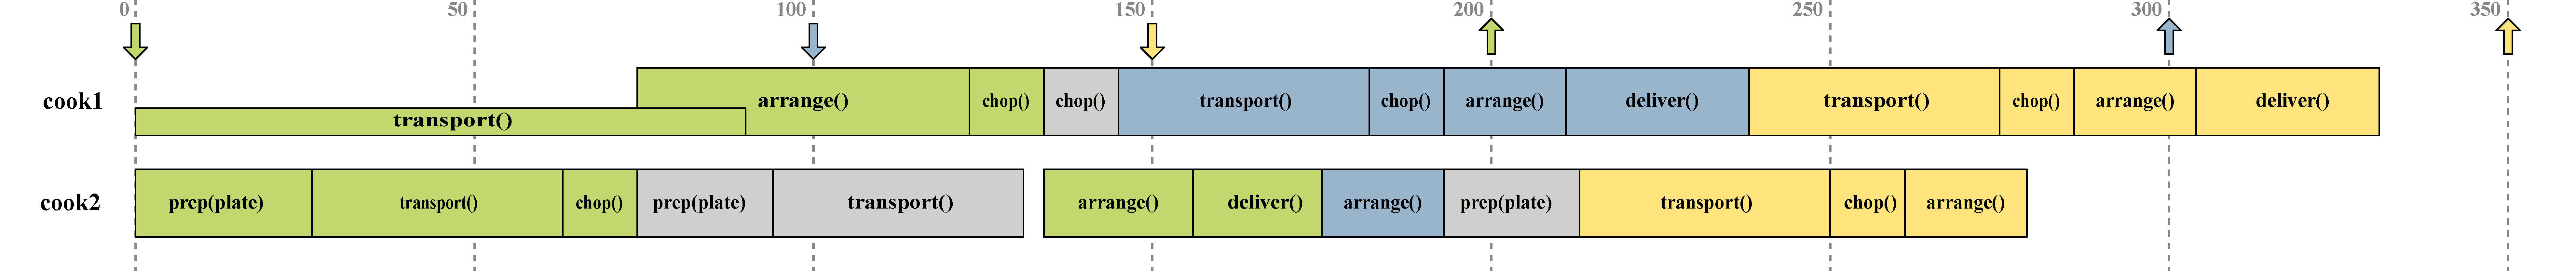
\includegraphics[width=\linewidth]{images/Scenario3 tomato - preparations.pdf}
    \end{minipage}
    \begin{minipage}{\textheight}
      \centering
      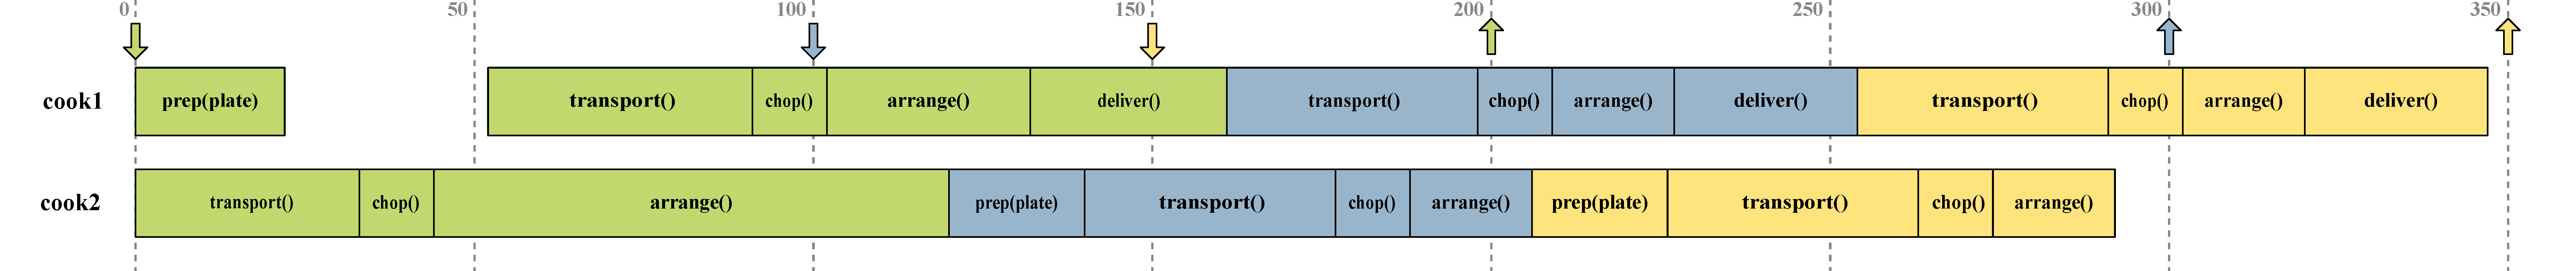
\includegraphics[width=\linewidth]{images/Scenario3 tomato - robustness.pdf}
    \end{minipage}
  \end{minipage}
  % \begin{figure}
  %   \centering
  %   \subfloat[With generic deliberation function]{\label{fig:background-acting-conceptual-deliberation}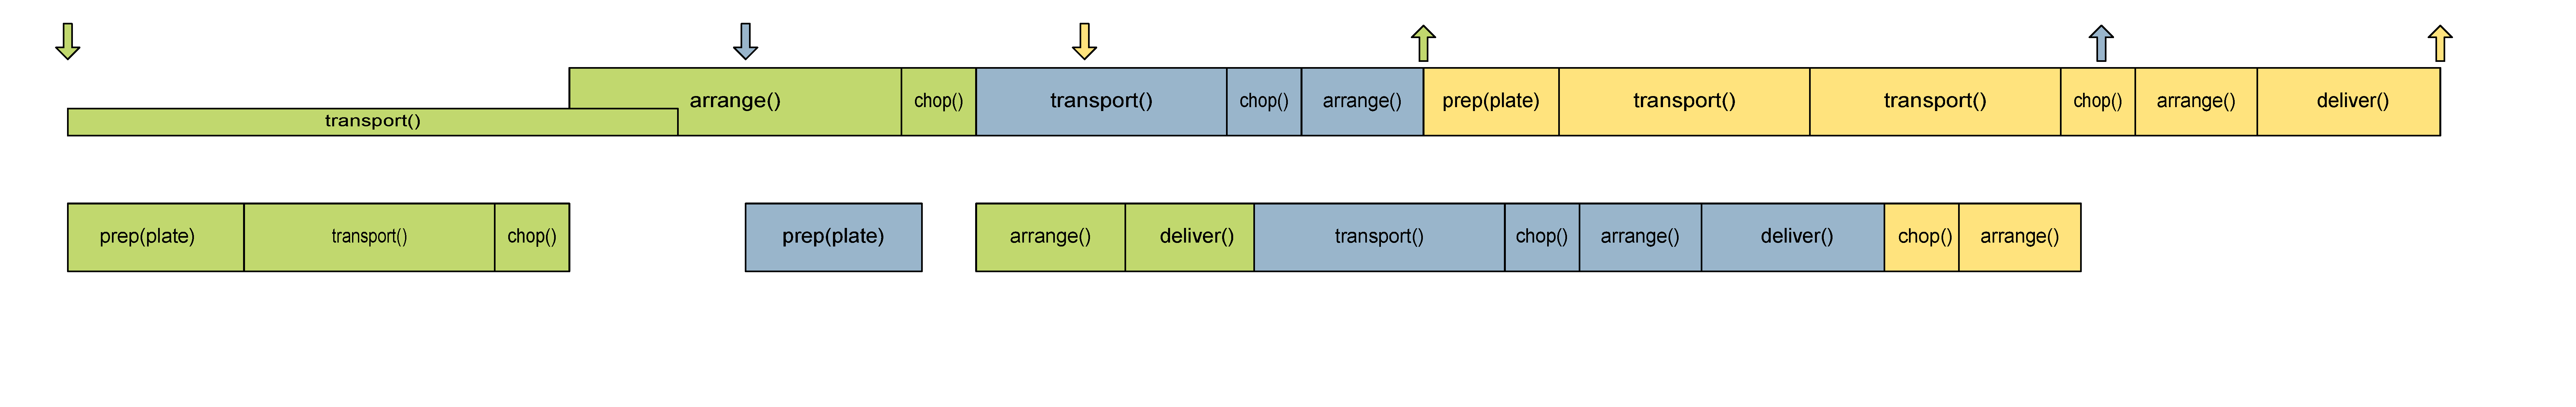
\includegraphics[width=0.4\textwidth]{images/Scenario3 tomato - default.pdf}}
  %   \subfloat[With only planning and acting]{\label{fig:background-acting-conceptual-pa}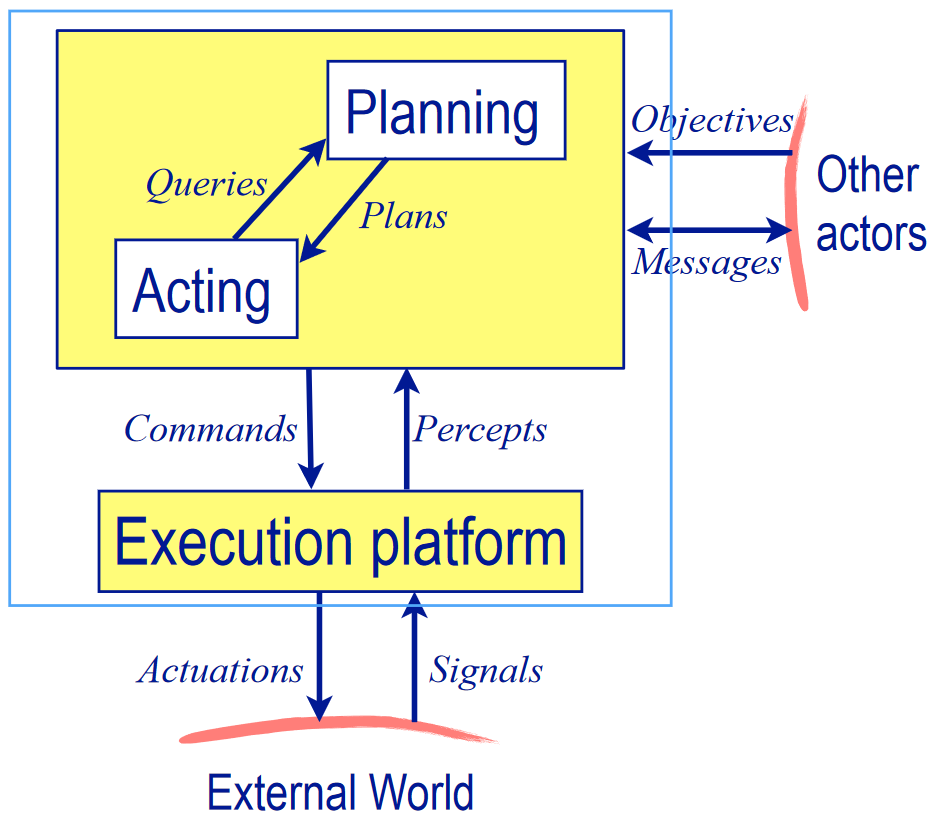
\includegraphics[width=0.4\textwidth]{images/background_acting_conceptual_p_a.png}}
  %   \caption[Conceptual view of an actor]{Conceptual view of an actor from \cite{ghallabAutomatedPlanningActing2016}}
  %   \label{fig:background-acting-conceptual}
  % \end{figure}
}